\chapter{考虑客流变化范围的鲁棒模型预测控制方法}\label{chap:04}

\setcounter{algorithm}{0} % 重置算法计数器

\section{问题描述}
\label{section2}

结合城际高速铁路的实际运行场景，本章内容组织如下：  
第~\ref{2.A} 节将实际的城际高速铁路环线抽象为数学模型；  
第~\ref{2.B} 节建立考虑客流不确定性的列车运行动态模型；  
第~\ref{2.C} 节基于前述动态模型构建状态空间模型；  
第~\ref{2.D} 节利用该状态空间模型建立鲁棒模型预测控制（MPC）问题。

\subsection{交通场景描述}
\label{2.A}

考虑一条连接两个端点城市 $A$ 与 $B$ 的双线城际高速铁路线路，沿线设有 $N$ 个中间车站，共有 $M$ 列列车投入运营（$M > N$）。所有列车采用“站站停”策略，在每一车站均停靠以服务上下车乘客。当列车抵达任一端点站后，立即折返并反向投入运营。

该线路采用高频次、地铁化的运营模式，无需越行或交叉操作，因此不考虑小交路（short-turning）或选择性跳站等调度策略。尽管城际铁路站间距相对较长，但在高峰时段，线路上运行的列车数量常超过车站数量 \citep{b44}。这种高密度部署可在保障全站通达性的前提下，提供高频率服务——这是以乘客为导向的运营核心目标之一。

此外，实际运行中通常无需越行操作，原因在于列车巡航速度高度同质化。若实施越行，还需配置专用基础设施（如越行线或额外轨道），而此类设施在城市或半城市化铁路环境中极为罕见。因此，排除越行假设与现代城际高速铁路系统的标准运营实践高度一致。

\begin{figure}
    \centering
    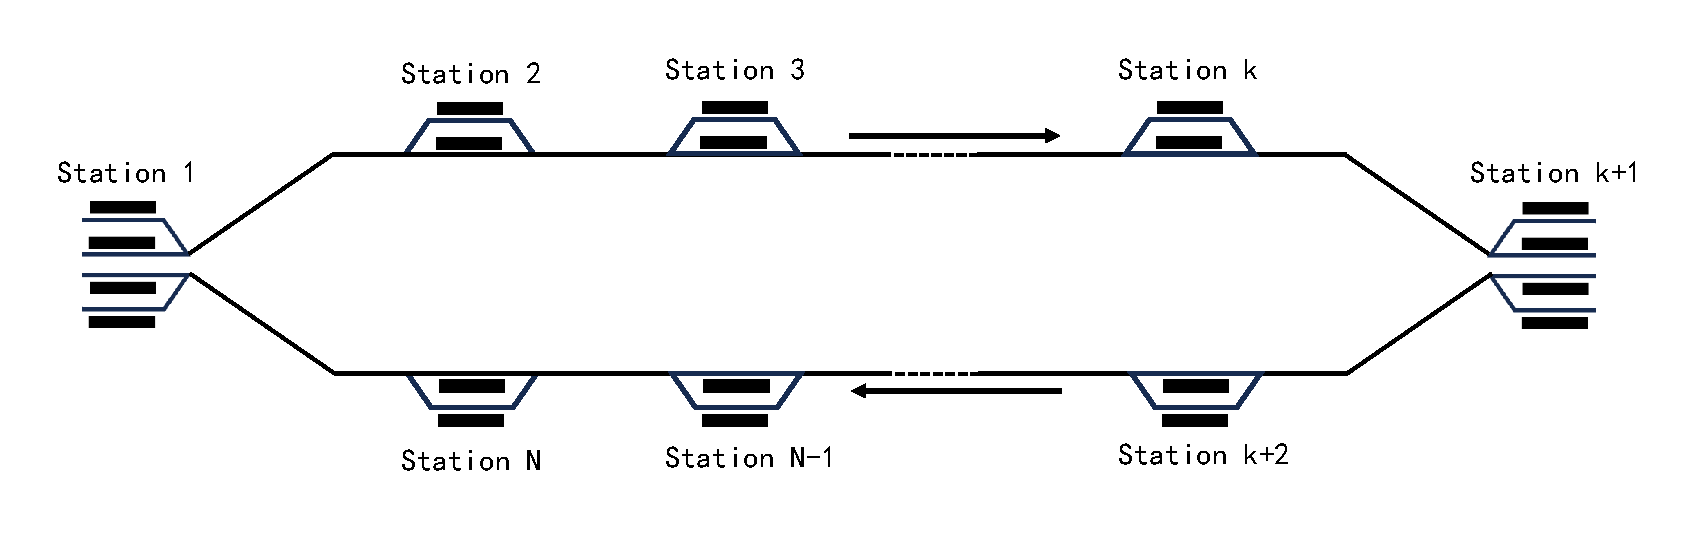
\includegraphics[width=\textwidth]{Img/Ch4/linestruct-mpc.pdf}
    \caption{城际高速铁路线路结构示意图}
    \label{fig:example}
\end{figure}

\textbf{环线模型}：环线定义为由 $N$ 个车站（编号从 1 至 $N$）组成的闭合线路，其中车站 $N$ 与车站 1 相连。一组列车（编号从 1 至 $M$）沿此环线周期性运行。各车站的列车出发顺序保持一致，列车依次停靠所有车站，其序列为：
\begin{equation*}
	\{1,2, \cdots, M, 1,2, \cdots, M, 1,2, \cdots\},
\end{equation*}
相应地，车站序列亦为：
\begin{equation*}
	\{1,2, \cdots, N, 1,2, \cdots, N, 1,2, \cdots\}.
\end{equation*}

由于高速铁路线路具有闭环结构，车站 1 处的列车状态变量演化不仅依赖于历史交通状况，还与前一站（即车站 $N$）的状态变量存在名义关联。需注意的是，当列车折返方式不同时，全线模型亦有所差异。在实际城际高速铁路运营中，通常存在两种折返方式：站前折返与站后折返。然而，针对这两种折返方式，均可建立统一模型。基于上述描述，可将实际城际高速铁路线路建模为含 $M$ 列列车的环形模型。随后，通过关联交通动态与客流关系建立列车交通模型，并在此基础上设计相应的鲁棒 MPC 控制器。表 1 列出了用于描述列车动态模型的关键变量。

\textbf{符号约定}：本文采用双下标记法标识与特定车站和列车相关的变量：下标表示车站编号，上标表示列车编号。这两个下标分别对 $N$ 和 $M$ 取模。据此约定，相邻两列列车可记为 $<i>$ 与 $<i+1>$（$1 \leq i \leq M$，其中列车 $<1>$ 紧随列车 $<M>$ 之后）；相邻两车站可记为 $<k>$ 与 $<k+1>$（$1 \leq k \leq N$，其中车站 $<1>$ 紧随车站 $<N>$ 之后）。

\subsection{列车交通动态方程}
\label{2.B}

根据城际高速铁路的实际运行情况，列车 $<i>$ 的出发时间演化可表示为 \citep{b18}：
\begin{equation}
   t_{k+1}^{i}=t_{k}^{i}+r_{k}^{i}+s_{k+1}^{i}
\label{equ:equ1}
\end{equation}
其中，$r_{k}^{i}$ 为列车 $<i>$ 从车站 $<k>$ 至 $<k+1>$ 的实际运行时间，$s_{k+1}^{i}$ 为列车 $<i>$ 在车站 $<k+1>$ 的停站时间。

区间实际运行时间可写为：
\begin{equation}
   r_{k}^{i}=R_{k}+u_{k}^{i}+w1_{k}^{i}
\label{equ:equ2}
\end{equation}
其中，$R_{k}$ 为时刻表规定的区间运行时间，$u_{k}^{i}$ 为列车 $<i>$ 在车站 $<k>$ 的出发时间调整量（即制定阶段调整计划时对 $R_k$ 的修正量），$w1_{k}^{i}$ 表示影响列车 $i$ 从车站 $k$ 至 $k+1$ 运行时间的不确定性干扰项。

停站时间可建模为：
\begin{equation}
    s_{k}^{i}=S+a\delta_{k} (t_{k}^{i}-t_{k}^{i-1})+w2_{k}^{i}
\label{equ:equ3}
\end{equation}
其中，$S$ 为车站最小停站时间，$a$ 为单位乘客平均上下车时间的影响系数，$\delta_{k}$ 为平均客流量，$w2_{k}^{i}$ 为影响停站时间的干扰项 \citep{b17}。前序列车的出发延误会影响当前列车的停站时间，而停站时间的变化又进一步影响当前列车的出发时间，从而形成列车间的相互耦合。

由式 \eqref{equ:equ3} 可知，客流量显著影响车站停站时间，进而直接影响出发时间。因此，客流波动可能导致调度延误。已有研究对城际高速铁路的客流分布进行了分析。例如，图 \ref{fig:passenger} 展示了京津城际高速铁路一日内的客流变化。分析表明，正态分布能较好拟合此类客流模式。

基于此，本文假设客流量服从正态分布，记为 $X \sim N(\mu, \sigma^2)$。该假设有助于更准确地预测潜在延误，并支撑鲁棒调度策略的设计。通过采用该模型，可深化对客流波动如何影响铁路运营的理解，从而提升高速铁路服务的效率与可靠性。

\begin{figure}
    \centering
    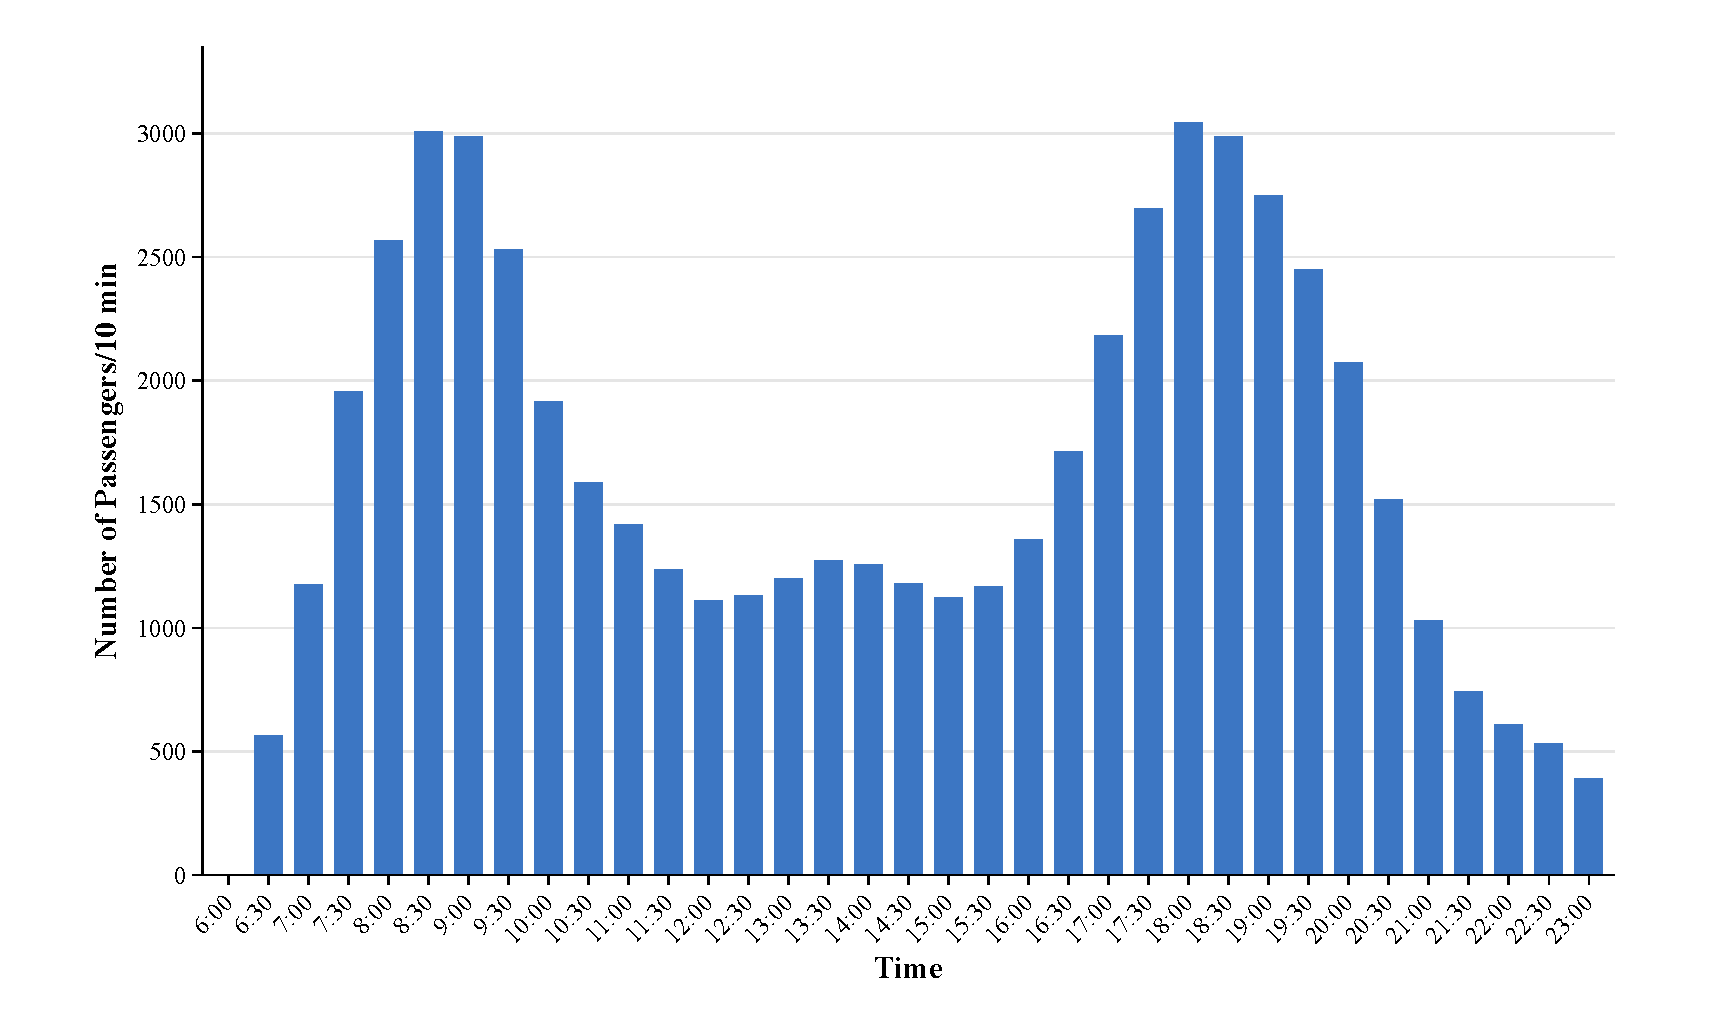
\includegraphics[width=\textwidth]{Img/Ch4/NumberofPassenger.pdf}
    \caption{京津城际高速铁路一日客流分布}
    \label{fig:passenger}
\end{figure}

\begin{figure}
    \centering
    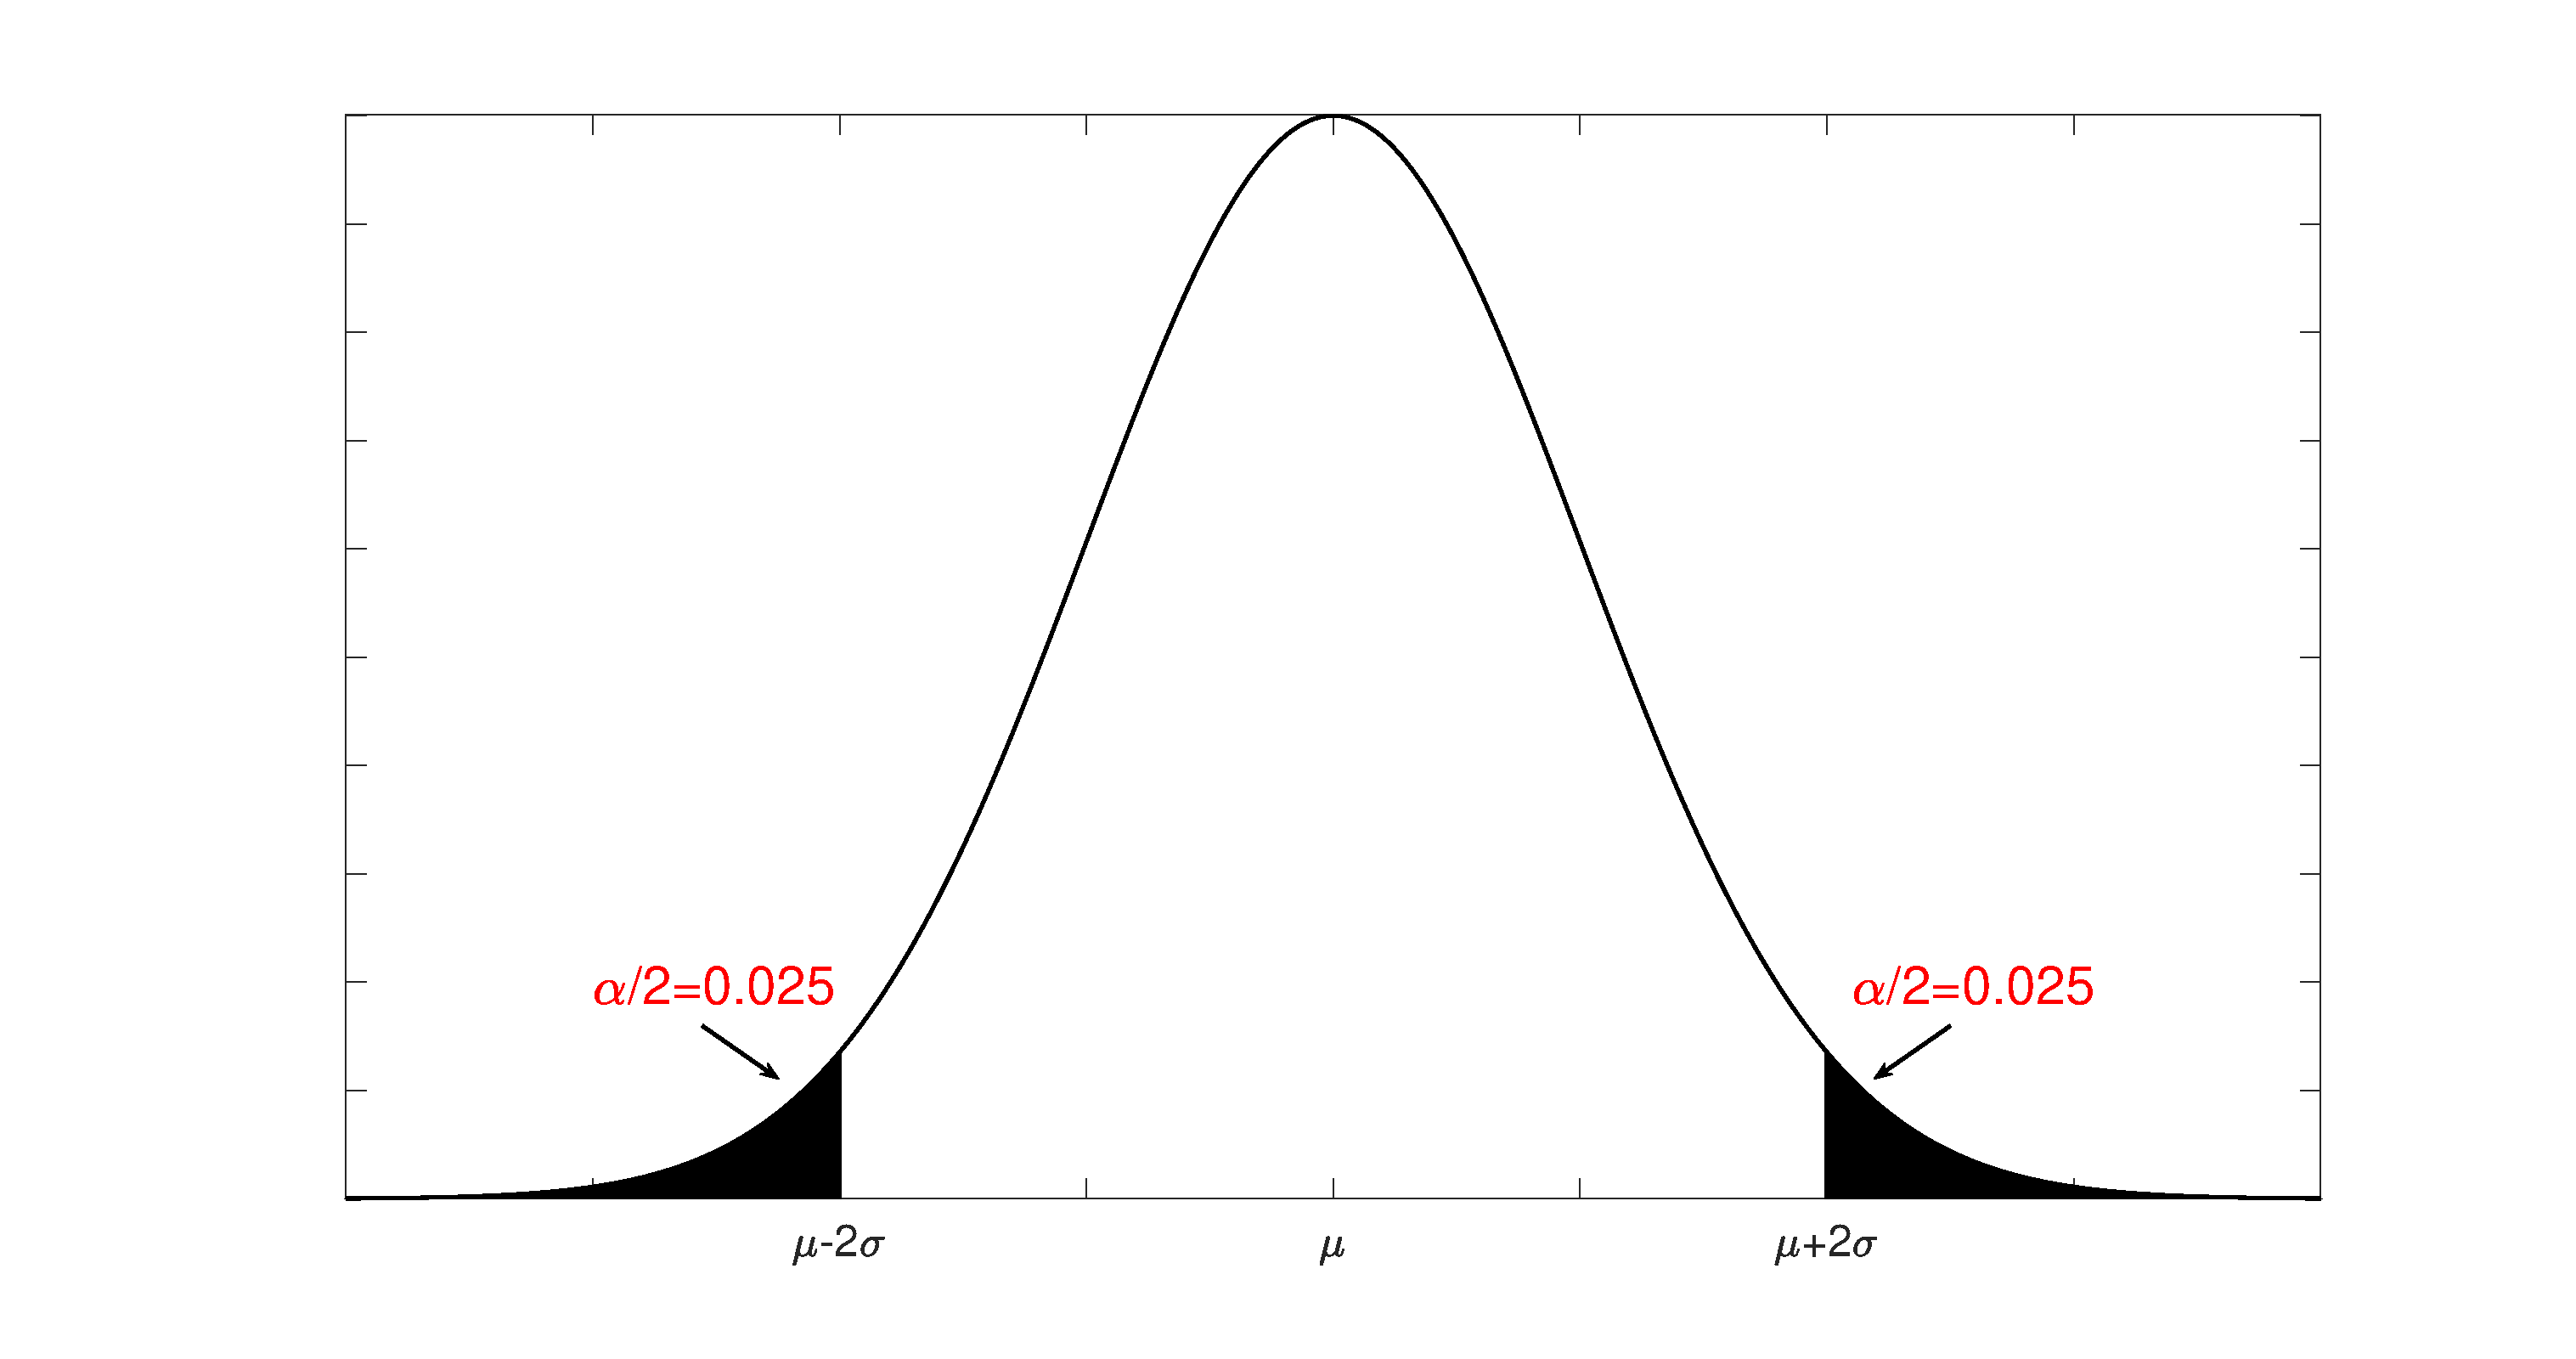
\includegraphics[width=\textwidth]{Img/Ch4/NormalDistribution.eps}
    \caption{客流分布的正态拟合}
    \label{fig:normal_dist}
\end{figure}

鉴于客流低于 $\mu - 2\sigma$ 或高于 $\mu + 2\sigma$ 的概率极低，此类事件可视为罕见且几乎不可能发生。因此，仅需考虑客流在 $[\mu - 2\sigma, \mu + 2\sigma]$ 范围内的变化。据此，可将客流变化范围设定为：
\begin{equation}
\delta_{k} = \delta + \alpha_{k} z, \quad -1 \leq \alpha_{k} \leq 1
\label{equ:equ4}
\end{equation}
其中，$\alpha_k$ 随车站变化；对每个车站，变化范围中心 $\delta = \mu$，半长 $z = 2\sigma$。

定义总干扰项为：
\begin{equation}
    w_{k}^{i} = w1_{k}^{i} + w2_{k+1}^{i}
\label{equ:equ5}
\end{equation}

联立式 (\ref{equ:equ1})–(\ref{equ:equ5})，可得：
\begin{equation}
    (1 - a\delta_{k+1}) t_{k+1}^{i} = t_{k}^{i} - a\delta_{k+1} t_{k+1}^{i-1} + S + R_{k} + u_{k}^{i} + w_{k}^{i}
\label{equ:equ6}
\end{equation}

在无控制与干扰（即 $u_{k}^{i} = w_{k}^{i} = 0$）情况下，时刻表出发时间 $T_{k}^{i}$ 应满足：
\begin{equation}
    T_{k+1}^{i} = T_{k}^{i} + a\delta_{k+1}( T_{k+1}^{i} - T_{k+1}^{i-1}) + S + R_{k}
\label{equ:equ7}
\end{equation}

令 $x_{k}^{i}$ 表示实际出发时间 $t_k^i$ 与时刻表出发时间 $T_{k}^{i}$ 的偏差，即：
\begin{equation}
    x_{k}^{i} = t_{k}^{i} - T_{k}^{i}
\label{equ:equ8}
\end{equation}

由式 (\ref{equ:equ6})–(\ref{equ:equ8}) 可得基本动态方程：
\begin{equation}
    (1 - a\delta_{k+1}) x_{k+1}^{i} + a\delta_{k+1} x_{k+1}^{i-1} = x_{k}^{i} + u_{k}^{i} + w_{k}^{i}, \quad k \geq 0,\ i \geq 1
\label{equ:equ9}
\end{equation}

\subsection{城际高速铁路状态空间模型}
\label{2.C}

为便于后续推导，首先定义四个形式化矩阵：

$D_{1}(a,b)$ 为 $M \times M$ 矩阵，结构如下：
\begin{equation*}
	D_{1}(a,b)=
	\begin{array}{ccccccccc}
		\setlength{\arraycolsep}{1mm}
		\left[
		\begin{array}{ccc|cccc}
			0&1& & & & & 0\\
			0&\ddots&\ddots & & & & \\
			& &0&1& & & \\ 
			\cline{1-7}
			0& & &a&b& & \\
			& & & &\ddots&\ddots& \\
			& & & & & a&b\\
			b& & & & & &a\\
		\end{array}
		\right]
		& 
		\begin{array}{c}
			\left.\rule{0mm}{3.5mm}\right\}M-N  \\ \hfill
			\\
			\\
			\left.\rule{0mm}{3.5mm}\right\}N \hfill
			\\
		\end{array} \\
		\begin{array}{cc}
			\underbrace{\rule{14mm}{0mm}}_{M-N} &  
			\underbrace{\rule{18mm}{0mm}}_{N}
		\end{array}
	\end{array}
\end{equation*}

$D_{2}(a)$ 为 $M \times N$ 矩阵，结构如下：
\begin{equation*}
	D_{2}(a)=
	\begin{array}{cccccc}
		\setlength{\arraycolsep}{1.5mm}
		\left[
		\begin{array}{ccc}
			& 0&  \\
			\cline{1-3}
			a& &0\\ 
			&\ddots & \\
			0& &a\\
			
		\end{array}
		\right]
		&  
		\begin{array}{c}
			\left.\rule{0mm}{2mm}\right\}M-N \\ 
			\\
			\left.\rule{0mm}{4mm}\right\}N \hfill\\
			\\
		\end{array}
	\end{array}
\end{equation*}

$D_{3}(a)$ 与 $D_{4}(a)$ 的结构类似，此处略去重复排版（实际使用时保留原矩阵图示）。

对每个车站 $<j>$，分别定义状态向量、控制向量与干扰向量：
\begin{gather}
    X_{j}^{i} = \big[ \underbrace{x_{j}^{i-M},\, x_{j}^{i-M+1},\, \dots,\, x_{j}^{i-N-1}}_{M-N},\ 
    \underbrace{x_{j}^{i-N},\, x_{j-1}^{i-N+1},\, \dots,\, x_{j-N+1}^{i-1}}_{N} \big]^{\!\!T} \notag \\ 
    U_{j}^{i} = \big[ \underbrace{u_{j-1}^{i-N+1},\, u_{j-2}^{i-N+2},\, \dots,\, u_{j-N}^{i}}_{N} \big]^{\!\!T} \notag \\ 
    W_{j}^{i} = \big[ \underbrace{w_{j-1}^{i-N+1},\, w_{j-2}^{i-N+2},\, \dots,\, w_{j-N}^{i}}_{N} \big]^{\!\!T}
    \label{equ:equ17}
\end{gather}

令 $\tilde{c}_{1,k} = \dfrac{-a\tilde{\delta}_k}{1 - a\tilde{\delta}_k}$，$\tilde{c}_{2,k} = \dfrac{1}{1 - a\tilde{\delta}_k}$。由统计数据可知 $0 < a \tilde{\delta}_{k} < 1$。基于式 (\ref{equ:equ4})，可将 $\tilde{c}_{1,k}$ 表示为：
\[
\tilde{c}_{1,k} = c_1 + \beta_{1,k} d_1, \quad -1 \leq \beta_{1,k} \leq 1,
\]
其中
\[
c_{1} = \frac{1}{2} \left( \frac{-a(\delta+z)}{1-a(\delta+z)} + \frac{-a(\delta-z)}{1-a(\delta-z)} \right), \quad
d_1 = \frac{1}{2} \left( \frac{-a(\delta-z)}{1-a(\delta-z)} - \frac{-a(\delta+z)}{1-a(\delta+z)} \right).
\]
类似地，
\[
\tilde{c}_{2,k} = c_2 + \beta_{2,k} d_2, \quad -1 \leq \beta_{2,k} \leq 1,
\]
其中
\[
c_{2} = \frac{1}{2} \left( \frac{1}{1-a(\delta+z)} + \frac{1}{1-a(\delta-z)} \right), \quad
d_2 = \frac{1}{2} \left( \frac{1}{1-a(\delta+z)} - \frac{1}{1-a(\delta-z)} \right).
\]

控制向量 $U_{j}^i$ 与干扰向量 $W_{j}^i$ 均为 $N$ 维向量，其元素与 $N$ 列列车相关，且上下标之和为定值。根据式 (\ref{equ:equ17})，由基本方程 (\ref{equ:equ9}) 可得状态空间方程：
\begin{equation}
\label{stateequation}
\begin{aligned}
X_{j}^{i+1} ={}& A X_{j}^{i} + I_{1} E_{1, j} C_{1} X_{j}^{i} + I_{1} E_{2, j} C_{2} X_{j}^{i} + B U_{j}^{i} \\
& + L E_{3, j} C_{3} U_{j}^{i} + B W_{j}^{i}, \quad j \in \{1,2, \ldots, N\}
\end{aligned}
\end{equation}
其中
\begin{align*}
&A = D_{1}(c_1, c_2), \quad B = D_{2}(c_1), \quad C_1 = D_3(d_1), \quad C_2 = D_4(d_2), \\
&I_{1} = I_{M \times M}, \quad L = D_2(1), \\
&E_{1,j} = \operatorname{diag}\big( \underbrace{\beta_{1,j}, \dots, \beta_{1,j}}_{M-N},\ \underbrace{\beta_{1,j}, \beta_{1,j-1}, \dots, \beta_{1,j-N+1}}_{N} \big), \\
&E_{2,j} = \operatorname{diag}\big( \underbrace{\beta_{2,j}, \dots, \beta_{2,j}}_{M-N},\ \underbrace{\beta_{2,j}, \beta_{2,j-1}, \dots, \beta_{2,j-N+1}}_{N} \big), \\
&E_{3,j} = \operatorname{diag}\big( \underbrace{\beta_{2,j}, \beta_{2,j-1}, \dots, \beta_{2,j-N+1}}_{N} \big), \\
&C_{3} = \operatorname{diag}\big( \underbrace{d_1, d_1, \dots, d_1}_{N} \big).
\end{align*}

由式 (\ref{stateequation}) 可知，各车站 $j$ 的误差状态空间模型结构不同，但均包含全线客流不确定性。因此，控制器设计过程具有一致性。不失一般性，可选取某一特定车站 $j_c \in \{1,2,\dots,N\}$ 进行设计。于是，误差状态空间模型 (\ref{stateequation}) 可简写为：
\begin{equation}
\label{model}
\begin{aligned}
X(i+1) ={}& A X(i) + I_{1} E_{1} C_{1} X(i) + I_{1} E_{2} C_{2} X(i) + B U(i) \\
& + L E_{3} C_{3} U(i) + B W(i), \quad i \in \{1,2, \ldots, M\}
\end{aligned}
\end{equation}

对于列车时刻表重调度问题，状态反馈控制律可表示为：
\begin{equation}
U(i) = K(i) X(i)
\end{equation}
其中 $K(i) \in \mathbb{R}^{N \times M}$ 为待求解的控制增益矩阵。

\subsection{鲁棒模型预测控制问题}
\label{2.D}

为保障列车运行性能，需在恢复时刻表的同时避免过度控制。当列车实际区段速度与正常运行速度偏差较大时，将导致频繁加减速，不仅增加能耗，也降低乘客舒适度。

定义如下代价函数：
\begin{equation}
G = \sum_{i=i_{0}}^{i_{f}} \left\{ X^{\!T}(i+1) Q X(i+1) + U^{\!T}(i) R U(i) \right\}
\end{equation}
其中，$Q$ 为 $M$ 维对角矩阵，前 $M-N$ 个元素为 0，其余元素为非负参数 $q$；$R$ 为 $N \times N$ 正定加权矩阵；$i_0$ 与 $i_f$ 分别为初始与终止状态序号。该代价函数的第一项惩罚 $N$ 列列车的时间偏差，第二项抑制控制量过大，整体目标是在恢复延误的同时避免过激调控。

基于代价函数 (\ref{costfunction})，考虑客流不确定性的城际高速铁路时刻表重调度鲁棒 MPC 问题可表述为：
\begin{equation}
	\label{costfunction}
	\begin{aligned}
		&\min_{U(i+j \mid i)=K(i) X(i+j \mid i),\ j=0,1,\dots,i_f-i} G(i) \\
		&= \sum_{j=0}^{i_f-i} \Big\{ X(i+j+1 \mid i)^{\!T} Q X(i+j+1 \mid i) \\
		&\qquad + U^{\!T}(i+j \mid i) R U(i+j \mid i) \Big\}
	\end{aligned}
\end{equation}
其中，$X(i+j \mid i)$ 为基于第 $i$ 步测量结果预测的第 $i+j$ 步误差状态，$U(i+j \mid i)$ 为第 $i$ 步优化问题计算出的第 $i+j$ 步控制量。

为确保重调度安全性，对控制量施加如下约束：
\begin{equation}
\label{constraint}
-\check{u} \leq U(i+j \mid i) \leq \hat{u}
\end{equation}
其中 $\check{u}$ 与 $\hat{u}$ 分别为控制输入的下限与上限。列车安全行车间隔由系统动态（特别是状态方程中前序列车状态 $x_{i-1}^{k+1}$ 的耦合项）与控制输入界 (\ref{constraint}) 共同隐式保证。若有必要，可显式添加最小行车间隔约束；但在本文框架下，动态耦合与有界控制已足以在常规工况下维持安全间隔。

综上，考虑客流不确定性与干扰的城际高速铁路时刻表重调度鲁棒 MPC 问题可采用 $H_\infty$ 控制方法求解。给定误差状态空间模型 (\ref{model})，需确定控制增益 $K(i)$，使其满足以下 $H_\infty$ 性能条件：

1) \textbf{延误恢复与调控目标}：当 $W(i) = 0$ 时，对所有允许的不确定性，代价函数 (\ref{costfunction}) 在约束 (\ref{constraint}) 下取得最小值；

2) \textbf{鲁棒性能}：以 $X(i) = 0$ 为初始条件，系统误差状态满足：
\begin{equation}
\begin{aligned}
\sum_{j=0}^{i_{f}-i} \big\| X(i+j+1 \mid i) \big\| \leq
\Gamma \sum_{j=0}^{i_{f}-i} \big\| W(i+j \mid i) \big\|,
\end{aligned}
\end{equation}
其中 $\Gamma > 0$ 为给定的扰动抑制水平。

\section{面向列车重调度的鲁棒模型预测控制器设计}
\label{section3}

本节基于前文提出的 $H_\infty$ 控制目标，提出一种适用于城际高速铁路时刻表重调度的鲁棒模型预测控制（Robust MPC）方法。所设计的控制增益 $K(i)$ 旨在同时实现两大目标：(1) 延误恢复与运能调整；(2) 鲁棒性能保障。

\subsection{延误恢复与运能调整目标}
为实现延误恢复与运能调整目标，需在干扰项 $W(i) = 0$ 的条件下，针对优化问题 (\ref{costfunction}) 设计相应的优化条件。

\textbf{定理 1：}考虑一条包含 $M$ 列列车、$N$ 个车站（$M > N$）的城际环线，假设 $W(i) = 0$，且各站客流满足模型 (\ref{model})。在每个决策步 $i$，状态反馈增益 $K(i)$ 在控制律 $U(i+j \mid i) = K(i) X(i+j \mid i)$（$j \geq 0$）中被精心设计，以最小化最坏情形下目标函数 $G(i)$ 的上界 $\alpha(i)$。

该控制增益可表示为 $K(i) = Y(i) Z^{-1}(i)$，其中矩阵 $Y(i)$ 与 $Z(i)$ 由以下线性矩阵不等式（LMI）组 (\ref{convexproblem})–(\ref{control2}) 的解确定：
\[
\Phi_{1}(i) = Z(i) A^{\!T} + Y^{\!T}(i) B^{\!T}, \quad
\Phi_{2}(i) = -Z(i) + \tilde{\theta}_{1}(i) I_{1} I_{1}^{\!T} + \tilde{\theta}_{2}(i) I_{1} I_{1}^{\!T} + \tilde{\theta}_{3}(i) L L^{\!T},
\]
\[
\bar{u}_{l} = \left( \frac{\hat{u}_{l} + \check{u}_{l}}{2} \right) - \left| \frac{\hat{u}_{l} - \check{u}_{l}}{2} \right|, \quad
H_{ll}(i) \text{ 为矩阵 } H(i) \text{ 的第 } l \text{ 个对角元素}.
\]

\begin{figure*}
    \begin{equation}
    \label{convexproblem}
    \min_{\substack{
        \tilde{\theta}_{1}(i)>0,\, \tilde{\theta}_{2}(i)>0,\, \tilde{\theta}_{3}(i)>0, \\
        \alpha(i)>0,\, Z(i)>0,\, Y(i)>0,\, H(i)>0
    }} \alpha(i)
    \end{equation}
    
    \begin{equation}
    \label{inequality1}
    \text{s.t.} \quad
    \begin{bmatrix}
    -Z(i) & \Phi_{1}(i) & Z C_{1}^{\!T} & Z C_{2}^{\!T} & Y^{\!T} C_{3}^{\!T} & Z & Y^{\!T} \\
    \Phi_{1}^{\!T} & \Phi_{2} & 0 & 0 & 0 & 0 & 0 \\
    C_{1} Z & 0 & -\tilde{\theta}_{1} I & 0 & 0 & 0 & 0 \\
    C_{2} Z & 0 & 0 & -\tilde{\theta}_{2} I & 0 & 0 & 0 \\
    C_{3} Y & 0 & 0 & 0 & -\tilde{\theta}_{3} I & 0 & 0 \\
    Z & 0 & 0 & 0 & 0 & -\alpha Q^{-1} & 0 \\
    Y & 0 & 0 & 0 & 0 & 0 & -\alpha R^{-1}
    \end{bmatrix} < 0
    \end{equation}
    
    \begin{equation}
    \label{maincondition2}
    \begin{bmatrix}
    1 & X(i) \\
    X^{\!T}(i) & Z(i)
    \end{bmatrix} \succeq 0
    \end{equation}
    
    \begin{equation}
    \label{control1}
    \begin{bmatrix}
    H(i) & Y(i) \\
    Y^{\!T}(i) & Z(i)
    \end{bmatrix} \succeq 0
    \end{equation}
    
    \begin{equation}
    \label{control2}
    H_{ll}(i) \leq U_{l}^{2}
    \end{equation}
    \hrulefill
    \vspace{-1em}
\end{figure*}

\textbf{证明：}为实现延误恢复目标，在决策步 $i$ 构造如下 Lyapunov 函数：
\begin{equation}
V(X(i)) = X^{\!T}(i) P X(i).
\end{equation}
首先假设满足如下鲁棒稳定性不等式：
\begin{equation}
\label{suppose}
\begin{aligned}
& V(X(i+j+1 \mid i)) - V(X(i+j \mid i)) \\
& \leq -\big[ X^{\!T}(i+j+1 \mid i) Q X(i+j+1 \mid i) + U^{\!T}(i+j \mid i) R U(i+j \mid i) \big],
\end{aligned}
\end{equation}
其中 $j = 0,1,\dots,i_f - i$。

对 $j$ 从 0 到 $i_f - i$ 求和，可得：
\begin{equation}
\begin{aligned}
G(i) &\leq V(X(i \mid i)) - V(X(i_f+1 \mid i)) \leq V(X(i \mid i)).
\end{aligned}
\end{equation}
令 $V(X(i \mid i)) \leq \alpha(i)$，则 $\alpha(i)$ 即为 $G(i)$ 的上界。通过变量替换 $Z(i) = \alpha(i) P^{-1}$，可将该约束转化为 LMI。

进一步，将系统动态 (\ref{model}) 代入 Lyapunov 差分，并结合控制律 $U = KX$，可得鲁棒稳定性条件 (\ref{condition})。利用 Schur 补引理与 Cauchy 不等式：
\[
A^{\!T}B + B^{\!T}A \leq \theta^{-1} A^{\!T}A + \theta B^{\!T}B, \quad \forall \theta > 0,
\]
可将含不确定性项 $E_1, E_2, E_3$ 的非线性项上界化，最终导出 LMI (\ref{inequality1})。

对于控制约束 (\ref{constraint})，其等价于：
\[
|U_l| \leq \frac{\hat{u}_l + \check{u}_l}{2} - \left| \frac{\hat{u}_l - \check{u}_l}{2} \right| =: U_l.
\]
结合 Cauchy-Schwarz 不等式与 LMI (\ref{control1})–(\ref{control2})，可保证该约束成立。

综上，当 $W(i) = 0$ 时，凸优化问题 (\ref{convexproblem}) 在约束 (\ref{inequality1})–(\ref{control2}) 下可高效求解 $\alpha(i)$ 的最小上界。由于该问题为 LMI 形式，可在多项式时间内求解 \citep{b45}，计算复杂度低，满足城际铁路实时重调度需求。

\subsection{鲁棒性能优化}
在完成延误恢复目标的基础上，进一步设计面向客流与运行干扰不确定性的鲁棒重调度方法。

\textbf{定理 2:} 给定常数 $\Gamma > 0$，在每个决策步 $i$，最小化目标函数 $G(i)$ 上界的 LMI 优化问题如下：
\begin{equation}
\label{inequality4}
\text{s.t. (\ref{inequality1})--(\ref{control2}), 且 }
\begin{bmatrix}
\varPi_1(i) & \varPi_2^{\!T}(i) \\
\varPi_2(i) & \varPi_3(i)
\end{bmatrix} < 0,
\end{equation}
其中 $\varPi_1(i), \varPi_2(i), \varPi_3(i)$ 如图~\ref{fig:my_label} 所示。求解该问题可得一组解 $\big[ \tilde{\theta}_1(i), \tilde{\theta}_2(i), \tilde{\theta}_3(i), \alpha(i), Z(i), Y(i), H(i) \big]$。采用鲁棒 MPC 控制律 $U(i+j \mid i) = Y(i) Z^{-1}(i) X(i+j \mid i)$，可同时实现：(1) 最小化延误恢复上界；(2) 对扰动 $W(i)$ 实现 $H_\infty$ 干扰抑制水平 $\Gamma$。


\textbf{证明：}由 Schur 补可知，当 LMI (\ref{inequality4}) 成立时，系统满足：
\begin{equation}
\begin{aligned}
& V(X(i+j+1 \mid i)) - V(X(i+j \mid i)) \\
& + \|X(i+j \mid i)\|^2 - \Gamma^2 \|W(i+j \mid i)\|^2 < 0.
\end{aligned}
\end{equation}
在初始状态 $X(i) = 0$ 下，对 $j = 0$ 至 $i_f - i$ 求和，可得：
\[
\sum_{j=0}^{i_f - i} \|X(i+j+1 \mid i)\| \leq \Gamma \sum_{j=0}^{i_f - i} \|W(i+j \mid i)\|,
\]
即满足 $H_\infty$ 鲁棒性能要求。

因此，所提鲁棒 MPC 控制器在客流不确定与外部干扰下，既能有效恢复时刻表，又具备强鲁棒性，适用于实际高密度城际铁路运营场景。


\section{仿真实验结果}
\label{section4}

为验证所提鲁棒 MPC 控制器的有效性，构建基于京津城际高速铁路的仿真系统。模型将实际 5 站线路抽象为 8 个车站，15 列列车在环线上运行。控制器代价函数 (\ref{costfunction}) 中的权重矩阵设为 $Q = 0.1 I_{15}$、$R = 0.1 I_8$。

客流参数基于历史数据设定：名义客流量 $\delta = 0.35$，波动半径 $z = 0.15$，单位乘客对停站时间影响系数 $a = 0.2$。选取 $H_\infty$ 干扰抑制水平 $\Gamma = 2.6$，控制量约束为 $-10~\text{分钟} \leq u_k^i \leq 15~\text{分钟}$。控制增益通过 MATLAB LMI 工具箱求解。

\subsection{案例一：客流不确定性干扰}
为验证控制器对客流不确定性的抑制能力，对比 FCFS（先到先服务）、终点站时间裕度法（Terminus Time Margin）与本文鲁棒 MPC 方法。

结果如图~\ref{fig3:FCFS}–\ref{fig5:Error} 所示。采用 FCFS 时，客流不确定性导致延误持续累积，至第 10 站（第二圈第 2 站），各列车延误已达约 7 分钟。而鲁棒 MPC 方法将所有列车延误始终控制在 1 分钟以内，显著优于其他两种方法，且调整速度更快。

\begin{figure}[htbp!]
\centering
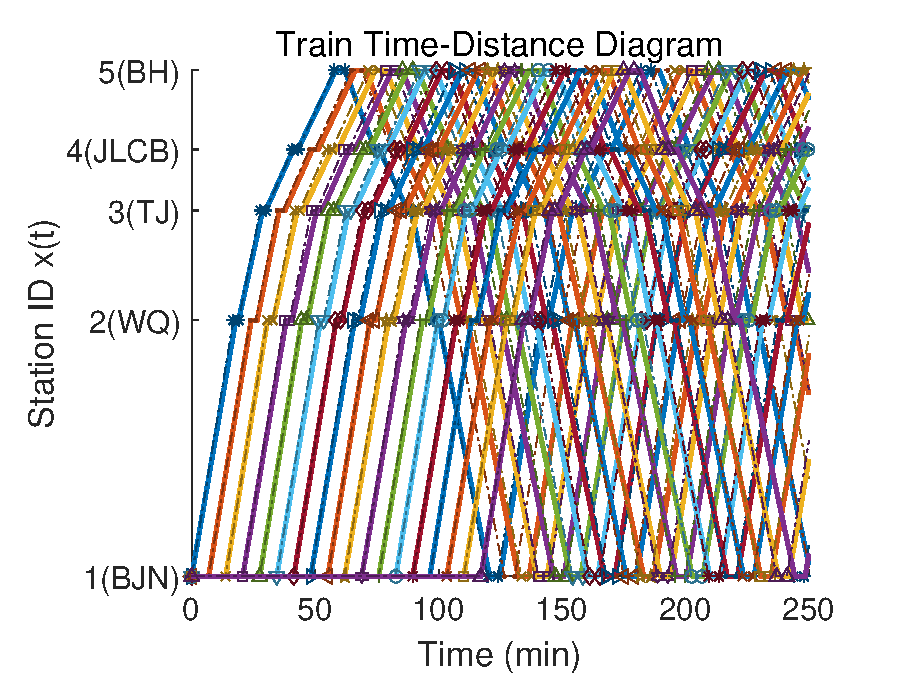
\includegraphics[width=\textwidth]{Img/Ch4/NOCONTROL.eps}
\caption{名义时刻表（虚线）与 FCFS 方法实际运行图（实线）}
\label{fig3:FCFS}
\end{figure}

\begin{figure}[htbp!]
\centering
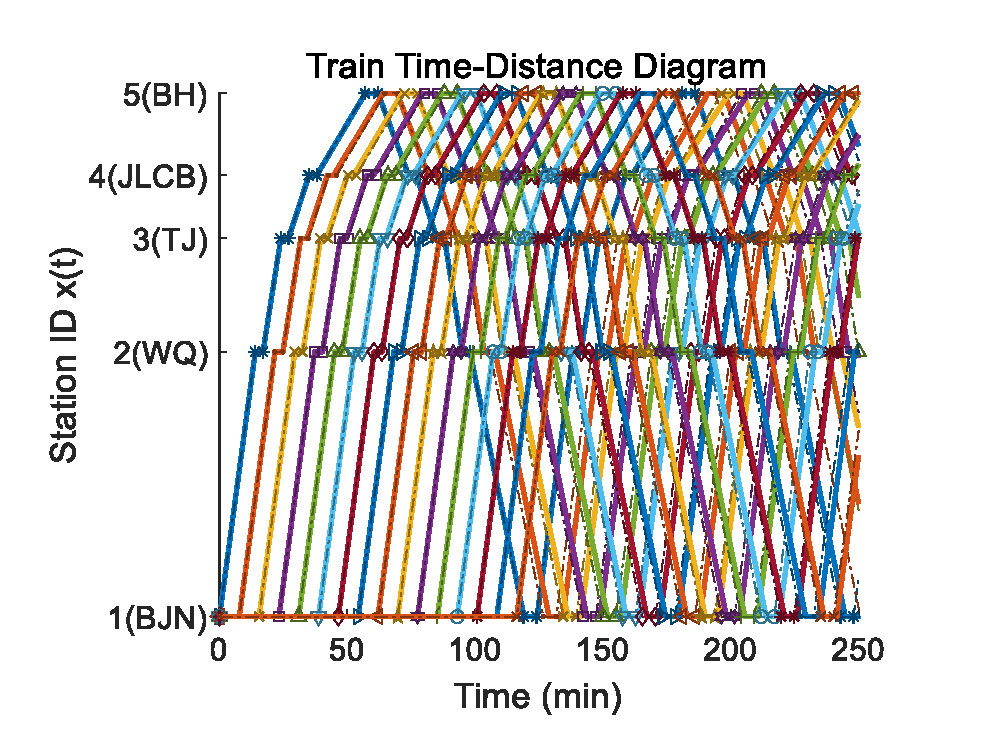
\includegraphics[width=\textwidth]{Img/Ch4/Human.pdf}
\caption{名义时刻表（虚线）与终点站时间裕度法实际运行图（实线）}
\label{fig:Termius}
\end{figure}

\begin{figure}[htbp!]
\centering
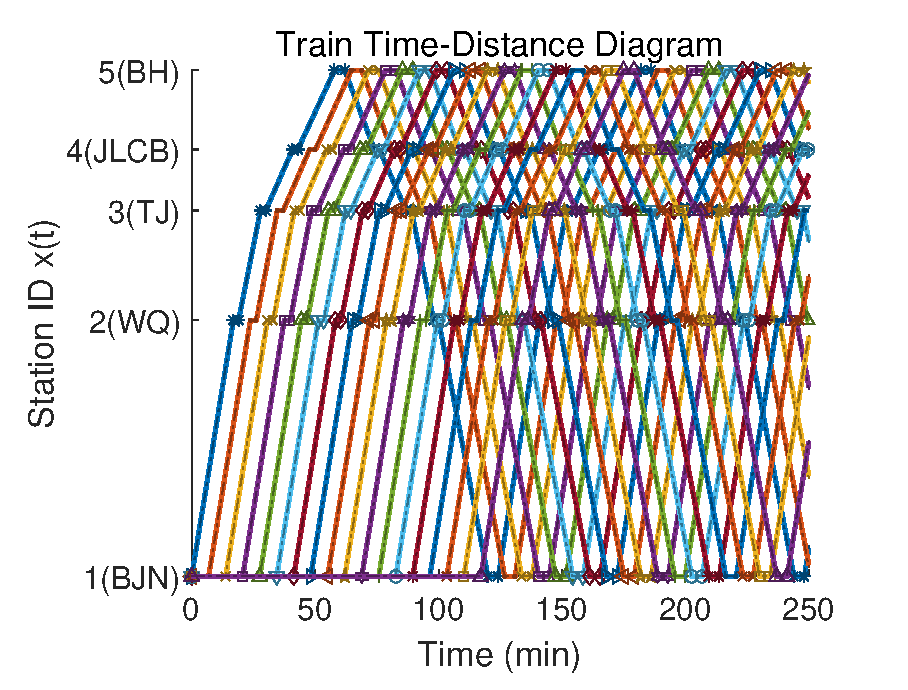
\includegraphics[width=\textwidth]{Img/Ch4/MPC.eps}
\caption{鲁棒 MPC 方法生成的重调度列车运行图}
\label{fig4:robust MPC}
\end{figure}

\begin{figure}[htbp!]
\centering
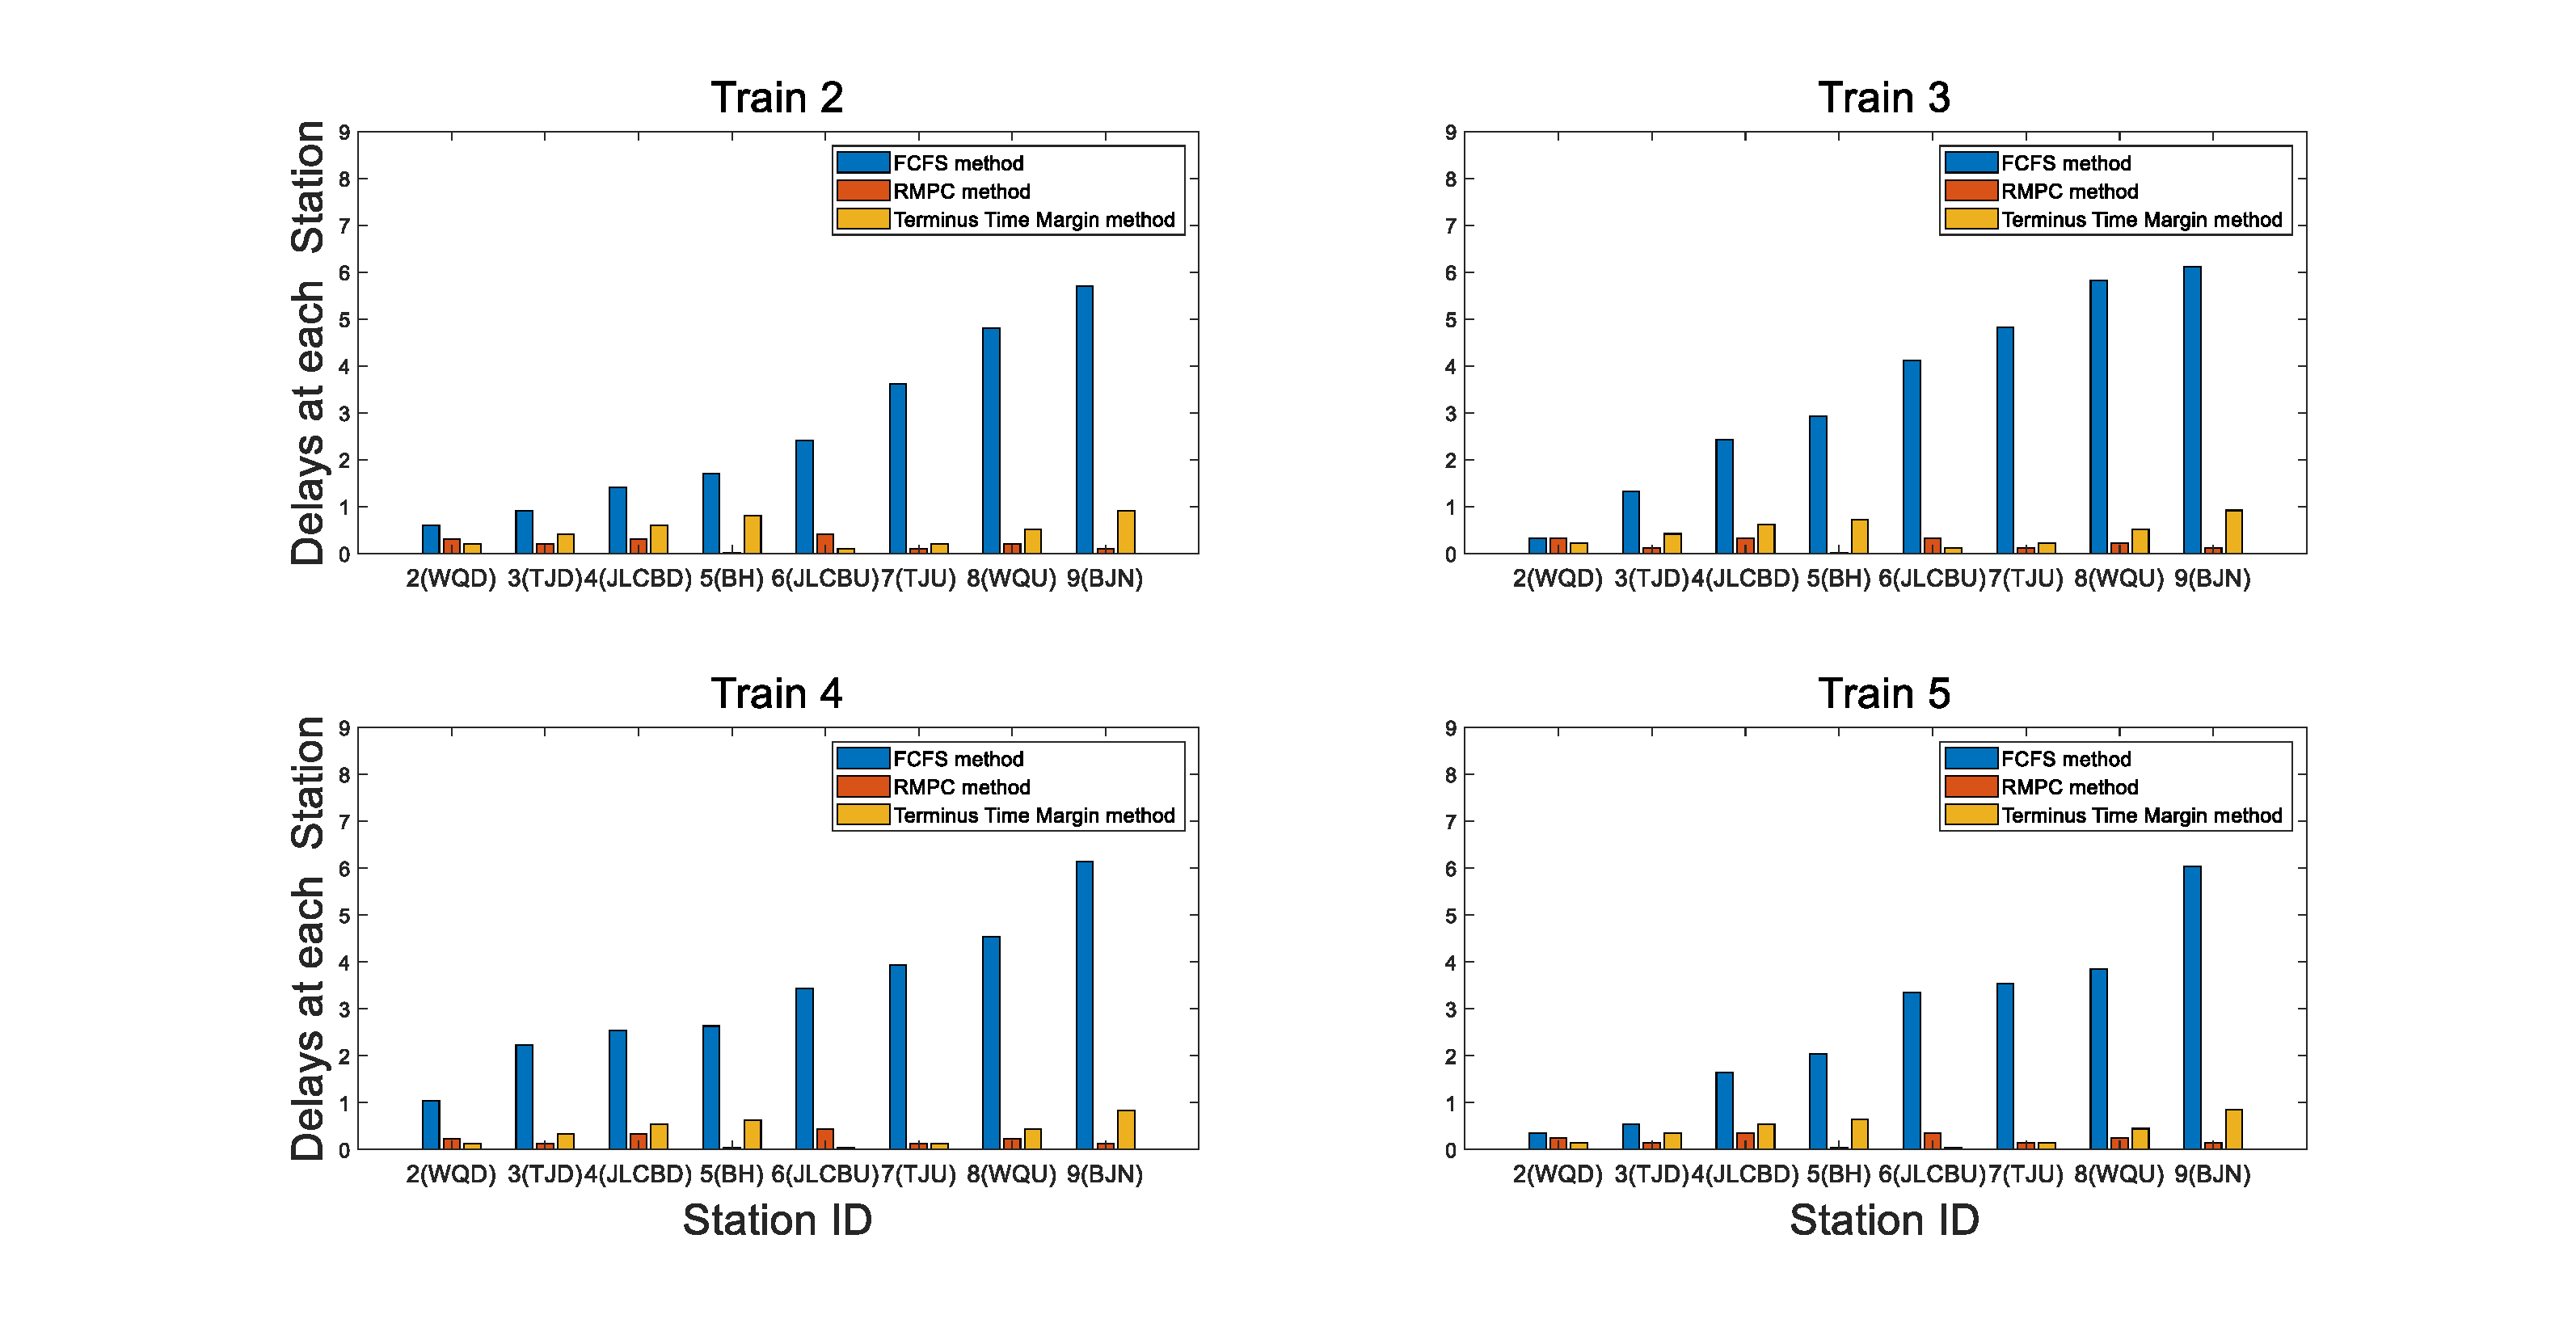
\includegraphics[width=\textwidth]{Img/Ch4/TreeConstrast.pdf}
\caption{列车 2–5 在各站的出发延误演化对比（FCFS vs 鲁棒 MPC）}
\label{fig5:Error}
\end{figure}

\subsection{案例二：突发大延误干扰}
假设列车 2 在车站 2 发生 15 分钟大延误，导致后续列车连锁延误（列车 3：12.4 分钟，列车 4：9.6 分钟，列车 5：6.3 分钟）。对比鲁棒 MPC、状态反馈控制器与混合整数规划（MIP）方法。

如图~\ref{fig6:robust MPC}–\ref{fig9:robust MPCError} 所示，鲁棒 MPC 在约 7 个车站后完全恢复时刻表；状态反馈控制器恢复较慢；MIP 因未考虑客流不确定性，导致后续延误逐渐扩大。

\begin{figure}[htbp!]
\centering
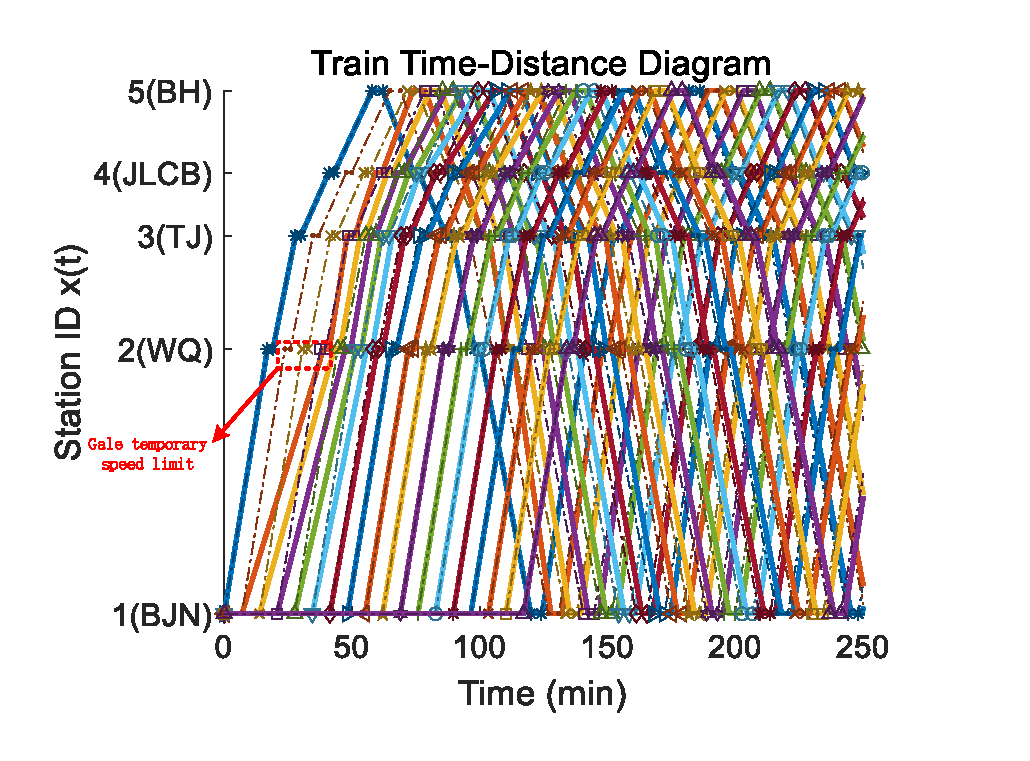
\includegraphics[width=\textwidth]{Img/Ch4/ControlError.pdf}
\caption{状态反馈控制器重调度结果}
\label{fig7:feedback}
\end{figure}

\begin{figure}[htbp!]
\centering
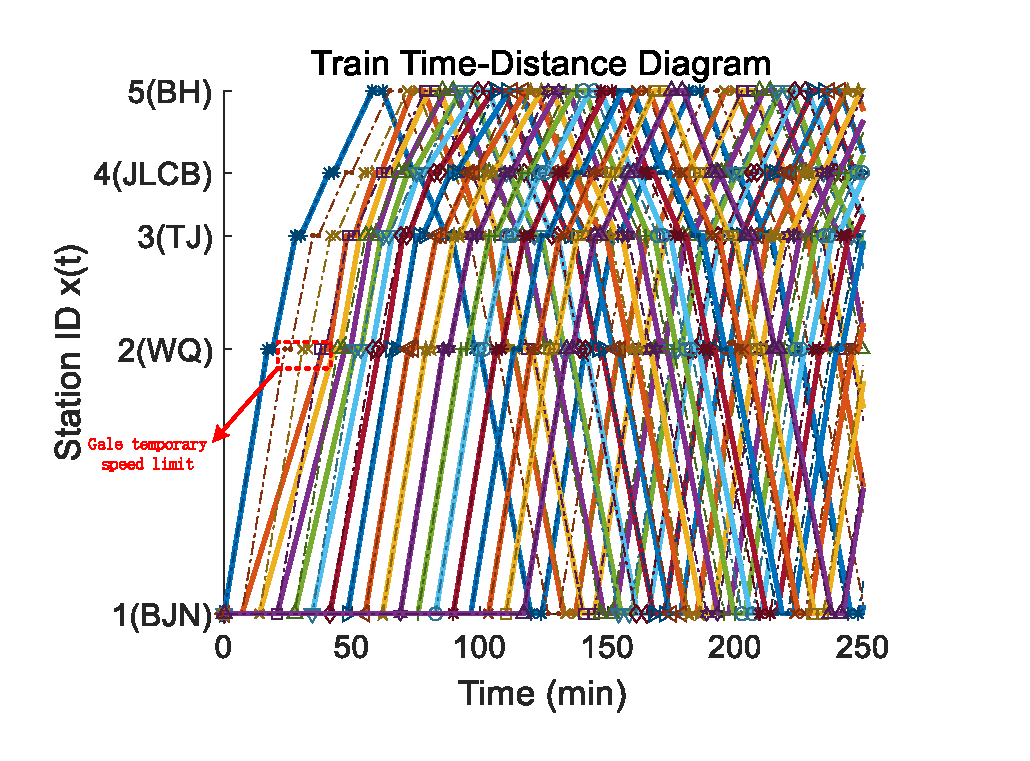
\includegraphics[width=\textwidth]{Img/Ch4/MIPError.pdf}
\caption{MIP 方法重调度结果}
\label{fig8:MIP}
\end{figure}

\begin{figure}[htbp!]
\centering
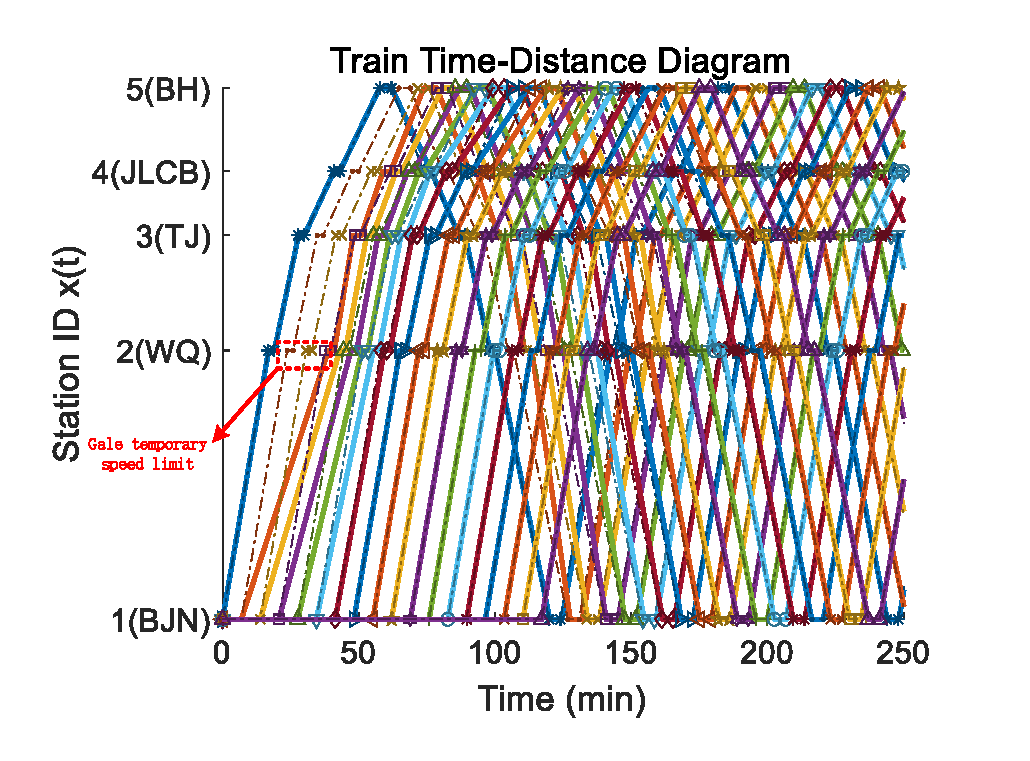
\includegraphics[width=\textwidth]{Img/Ch4/rmpcError.pdf}
\caption{鲁棒 MPC 方法重调度结果}
\label{fig6:robust MPC}
\end{figure}

\begin{figure}[htbp!]
\centering
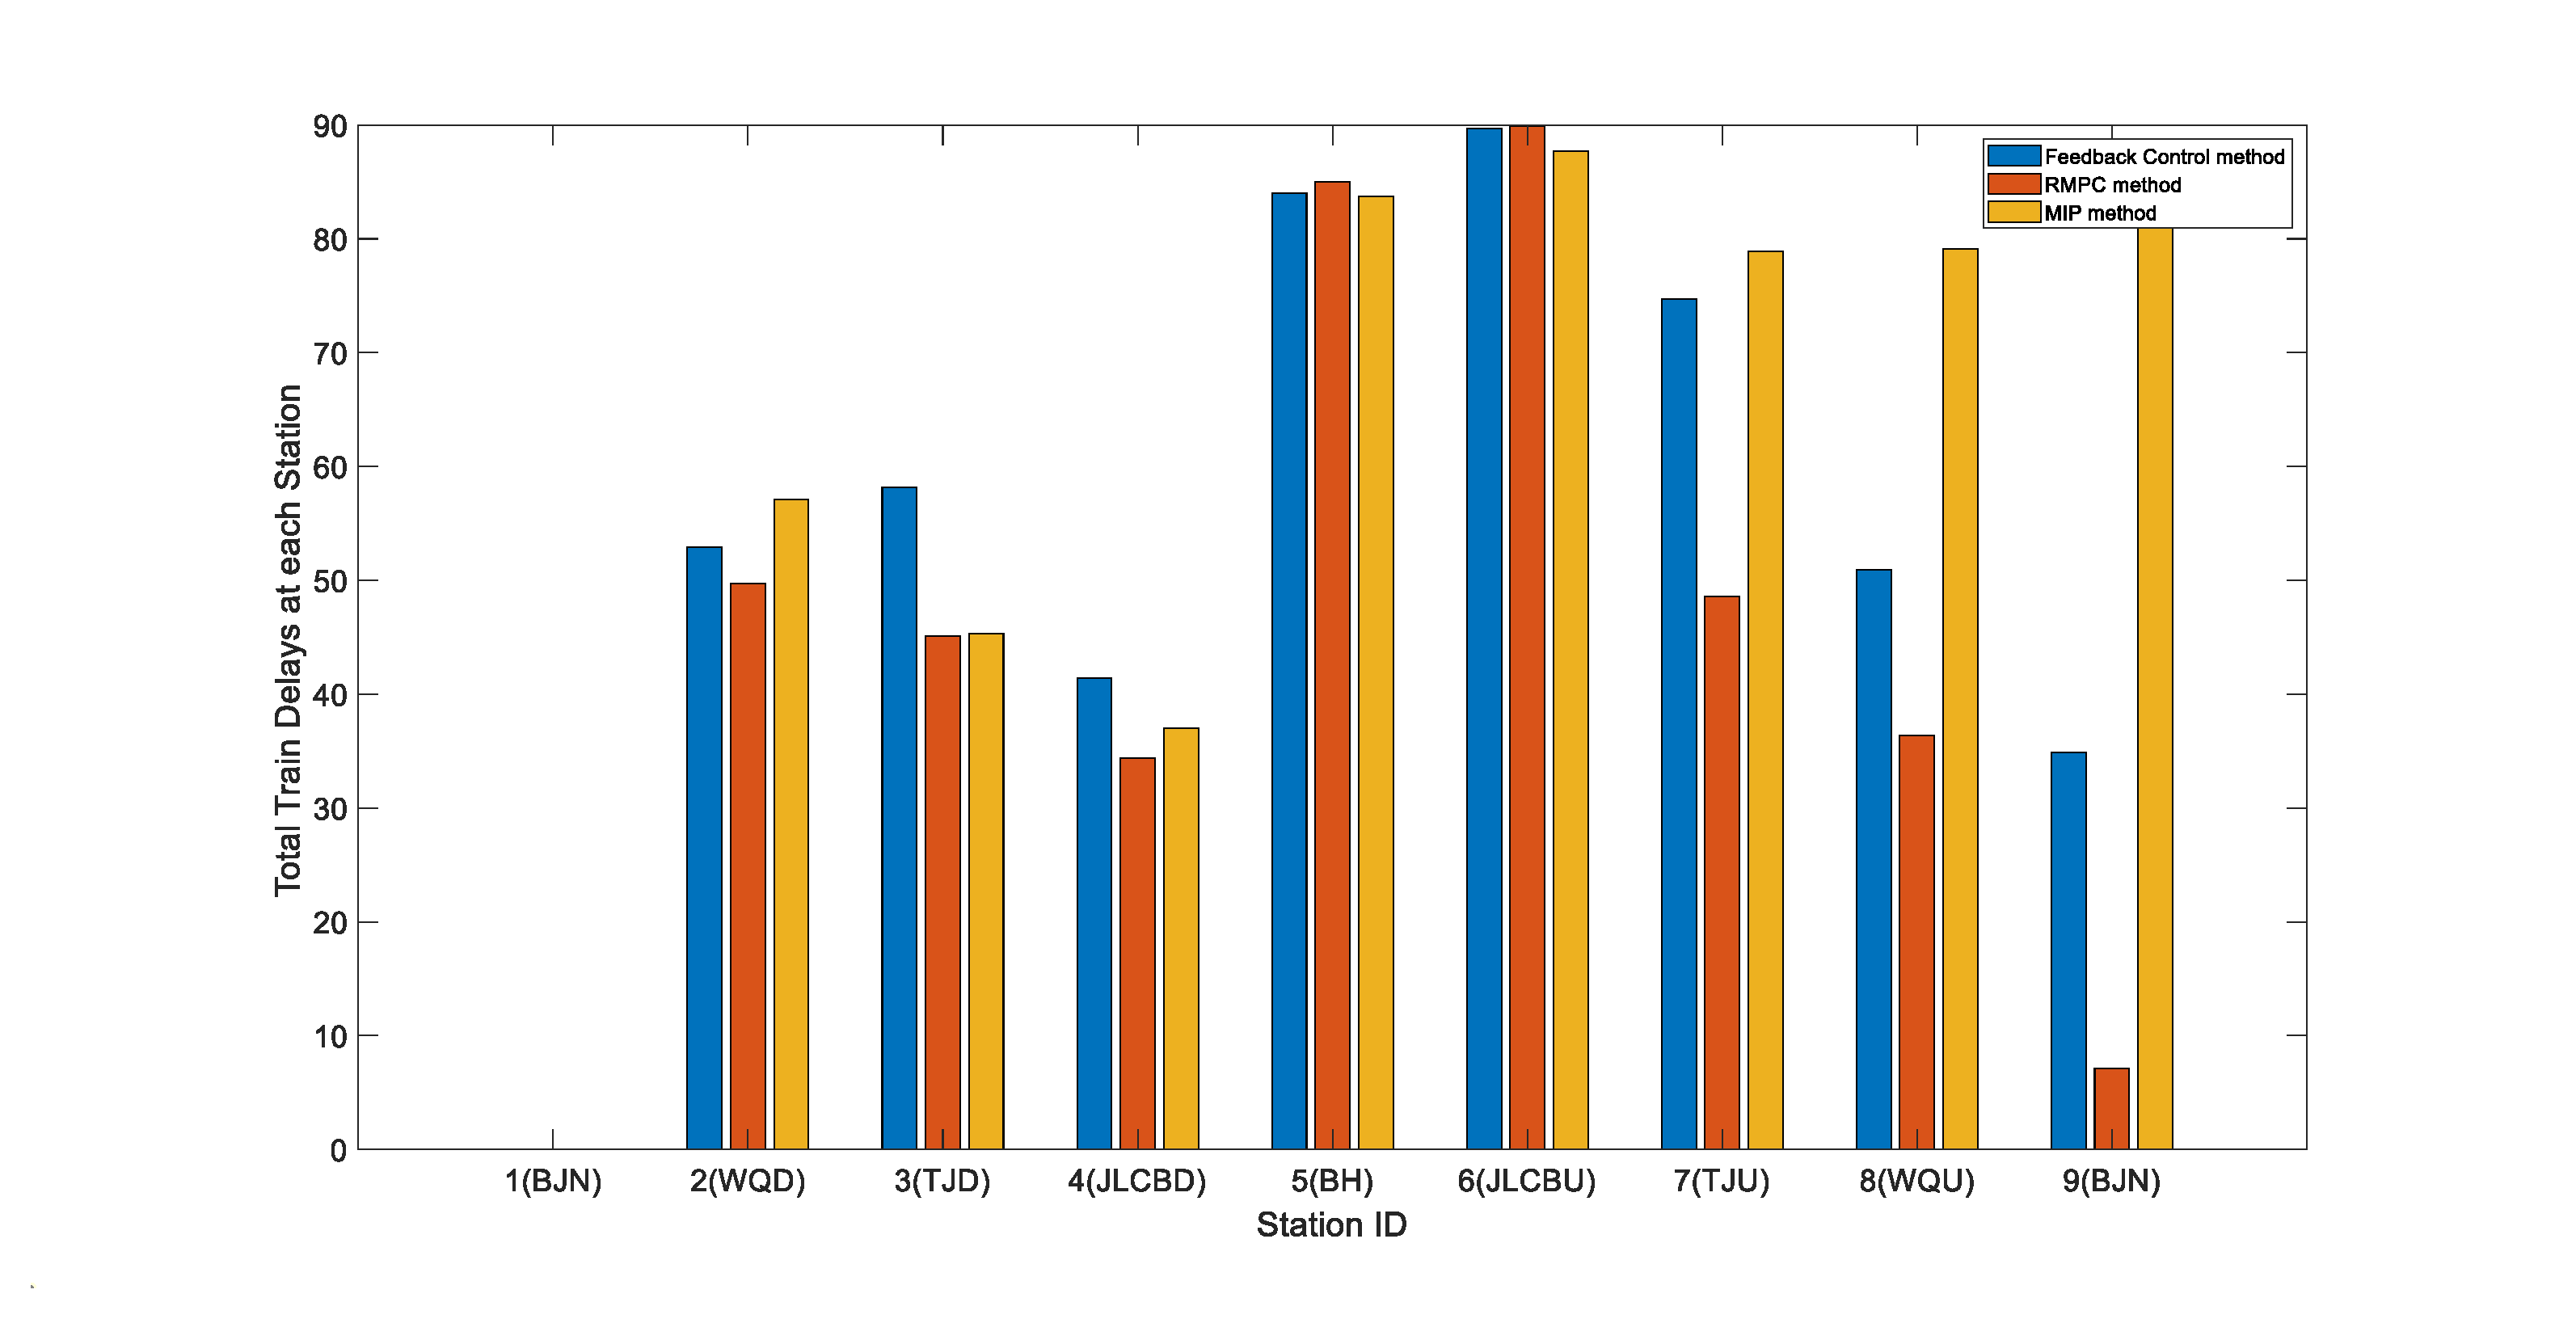
\includegraphics[width=\textwidth]{Img/Ch4/Errorcontrast.pdf}
\caption{三种方法的列车延误演化对比}
\label{fig9:robust MPCError}
\end{figure}

\begin{figure}[htbp!]
\centering
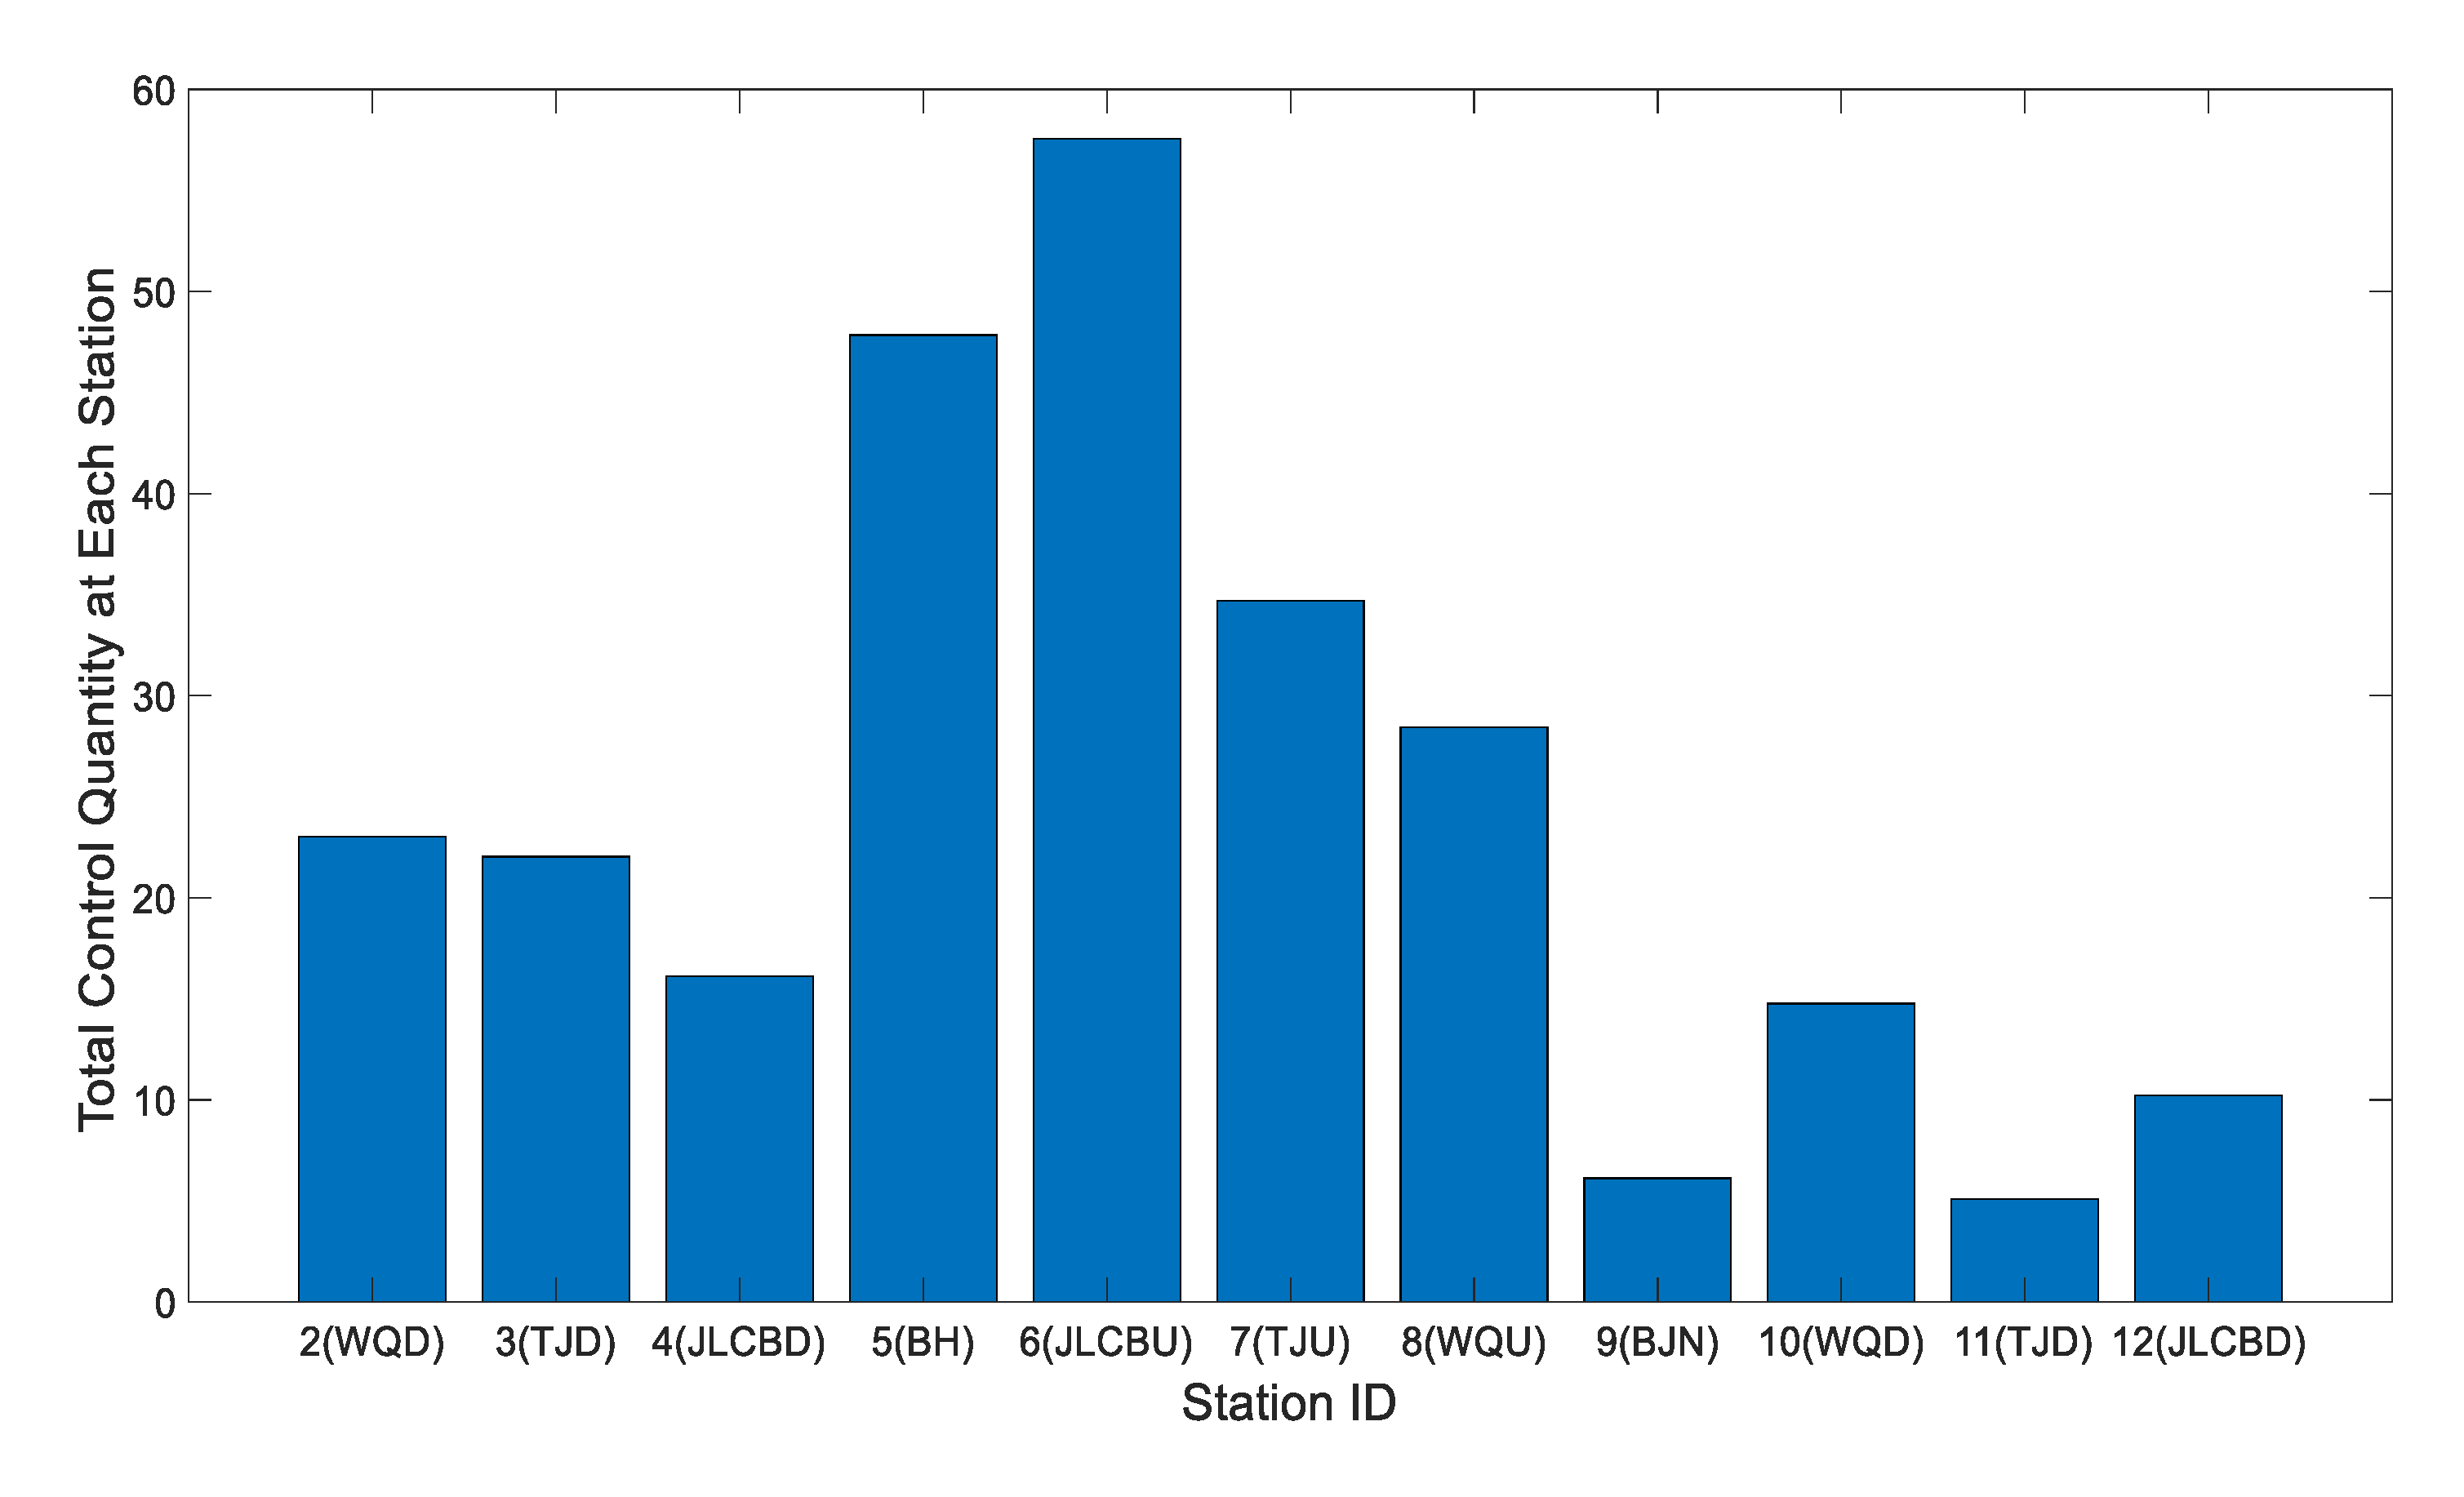
\includegraphics[width=\textwidth]{Img/Ch4/ControlMPC.pdf}
\caption{鲁棒 MPC 控制量随时间演化}
\label{fig:control_mpc}
\end{figure}

\begin{table}[!htbp]
\centering
\caption{不同规模下鲁棒 MPC 的计算时间}     
\label{computation time}
\begin{tabular}{ccc}
\hline
列车数 & 车站数 & 计算时间 (s) \\
\hline
16 & 8  & 5.17  \\
18 & 10 & 7.22  \\
20 & 12 & 11.51 \\
22 & 14 & 13.79 \\
24 & 16 & 20.34 \\
26 & 18 & 23.58 \\
\hline
\end{tabular}
\end{table}

由图~\ref{fig6:robust MPC} 可见，鲁棒 MPC 能有效收敛延误至零；图~\ref{fig9:robust MPCError} 显示其性能比状态反馈控制器提升 25.3\%。表~\ref{computation time} 表明，即使在 26 列车、18 车站的高密度场景下，计算时间仍低于 24 秒，满足实时性要求。

综上，所提鲁棒 MPC 控制器在抑制客流不确定性与突发干扰方面表现优异，兼具高性能与强实时性，适用于未来高密度城际铁路智能调度系统。

\section{本章小结}
\label{section5}

本章围绕城际高速铁路列车的状态空间建模与重调度控制问题展开研究，重点考虑了客流不确定性及运行干扰的影响。首先，通过推导城际高速列车的动力学方程，定义了合适的状态变量与控制变量，构建了事件触发机制下的状态空间模型。在此基础上，针对运行过程中的不确定性因素，设计了一种鲁棒模型预测控制（Robust Model Predictive Control, RMPC）算法用于列车时刻表重调度。该算法以最小化系统目标函数的上界为目标，同时保证对不确定性干扰的有效抑制。

为验证所提方法的有效性，将该鲁棒模型预测控制算法应用于城际高速铁路仿真车站场景，并与状态反馈控制方法及混合整数规划（MIP）方法进行了对比。仿真结果表明，所提出的方法在重调度性能方面具有明显优势。此外，该算法具备良好的可扩展性，可进一步推广至包含线路汇合与分岔的复杂城际铁路网络。未来工作将聚焦于分布式鲁棒模型预测控制算法的研究，以支持更大规模城际高速铁路网络的协同调度与结构优化。